\documentclass[]{article}
\usepackage{lmodern}
\usepackage{amssymb,amsmath}
\usepackage{ifxetex,ifluatex}
\usepackage{fixltx2e} % provides \textsubscript
\ifnum 0\ifxetex 1\fi\ifluatex 1\fi=0 % if pdftex
  \usepackage[T1]{fontenc}
  \usepackage[utf8]{inputenc}
\else % if luatex or xelatex
  \ifxetex
    \usepackage{mathspec}
  \else
    \usepackage{fontspec}
  \fi
  \defaultfontfeatures{Ligatures=TeX,Scale=MatchLowercase}
\fi
% use upquote if available, for straight quotes in verbatim environments
\IfFileExists{upquote.sty}{\usepackage{upquote}}{}
% use microtype if available
\IfFileExists{microtype.sty}{%
\usepackage{microtype}
\UseMicrotypeSet[protrusion]{basicmath} % disable protrusion for tt fonts
}{}
\usepackage[margin=1in]{geometry}
\usepackage{hyperref}
\hypersetup{unicode=true,
            pdftitle={Revisiting advice on the analysis of count data},
            pdfauthor={Michael B. Morrissey and Graeme D. Ruxton},
            pdfborder={0 0 0},
            breaklinks=true}
\urlstyle{same}  % don't use monospace font for urls
\usepackage{graphicx,grffile}
\makeatletter
\def\maxwidth{\ifdim\Gin@nat@width>\linewidth\linewidth\else\Gin@nat@width\fi}
\def\maxheight{\ifdim\Gin@nat@height>\textheight\textheight\else\Gin@nat@height\fi}
\makeatother
% Scale images if necessary, so that they will not overflow the page
% margins by default, and it is still possible to overwrite the defaults
% using explicit options in \includegraphics[width, height, ...]{}
\setkeys{Gin}{width=\maxwidth,height=\maxheight,keepaspectratio}
\IfFileExists{parskip.sty}{%
\usepackage{parskip}
}{% else
\setlength{\parindent}{0pt}
\setlength{\parskip}{6pt plus 2pt minus 1pt}
}
\setlength{\emergencystretch}{3em}  % prevent overfull lines
\providecommand{\tightlist}{%
  \setlength{\itemsep}{0pt}\setlength{\parskip}{0pt}}
\setcounter{secnumdepth}{0}
% Redefines (sub)paragraphs to behave more like sections
\ifx\paragraph\undefined\else
\let\oldparagraph\paragraph
\renewcommand{\paragraph}[1]{\oldparagraph{#1}\mbox{}}
\fi
\ifx\subparagraph\undefined\else
\let\oldsubparagraph\subparagraph
\renewcommand{\subparagraph}[1]{\oldsubparagraph{#1}\mbox{}}
\fi

%%% Use protect on footnotes to avoid problems with footnotes in titles
\let\rmarkdownfootnote\footnote%
\def\footnote{\protect\rmarkdownfootnote}

%%% Change title format to be more compact
\usepackage{titling}

% Create subtitle command for use in maketitle
\newcommand{\subtitle}[1]{
  \posttitle{
    \begin{center}\large#1\end{center}
    }
}

\setlength{\droptitle}{-2em}

  \title{Revisiting advice on the analysis of count data}
    \pretitle{\vspace{\droptitle}\centering\huge}
  \posttitle{\par}
    \author{Michael B. Morrissey and Graeme D. Ruxton}
    \preauthor{\centering\large\emph}
  \postauthor{\par}
      \predate{\centering\large\emph}
  \postdate{\par}
    \date{17 July, 2019}

\usepackage{fancyhdr}
\usepackage{lastpage}

\pagestyle{fancy}
\chead{~~~~~~~Simple models for count data}
\lhead{M.B. Morrissey and G.D. Ruxton}
\rhead{\thepage}
\renewcommand\headrulewidth{0.4pt}
\makeatletter
\let\ps@plain\ps@fancy
\makeatother
\usepackage{lineno}
\linenumbers
\usepackage{setspace}
\doublespacing
\usepackage{array}
\newcolumntype{x}[1]{>{\centering\arraybackslash\hspace{0pt}}p{#1}}
\usepackage{tabularx}
\usepackage{booktabs}
\usepackage{longtable}
\usepackage{array}
\usepackage{multirow}
\usepackage[table]{xcolor}
\usepackage{wrapfig}
\usepackage{float}
\usepackage{colortbl}
\usepackage{pdflscape}
\usepackage{tabu}
\usepackage{threeparttable}
\usepackage{threeparttablex}
\usepackage[normalem]{ulem}
\usepackage{makecell}

\begin{document}
\maketitle

Dyers Brae House

School of Biology

University of St Andrews

St Andrews, Scotland, KY16 9TH

\texttt{michael.morrissey@st-andrews.ac.uk}

\texttt{graeme.ruxton@st-andrews.ac.uk}

Author contributions: MBM and GDR both contributed to identifying the
key issue discussed in this paper, to constructing instructive scenarios
to illustrate the issue, to developing our re-interpretation of the
earlier results, and to writing the manuscript.

\clearpage

\subsection{Abstract}\label{abstract}

\begin{enumerate}
\def\labelenumi{(\arabic{enumi})}
\item
  O'Hara and Kotze (2010; Methods in Ecology and Evolution 1: 118-122)
  present simulation results that appear to show very poor behaviour (as
  judged by bias and overall accuracy) of linear models (LMs) applied to
  count data, especially in relation to generalised linear model (GLM)
  analysis.
\item
  We considered O'Hara and Kotze's (2010) comparisons, and determined
  that the finding occurred primarily because the quantity that they
  estimated in their simulations of the LM analysis (the mean of a
  transformation of the count data) was not the same quantity that was
  simulated and to which the results were compared (the logarithm of the
  mean of the count data). We correct this discrepancy, re-run O'Hara
  and Kotze's simulations, and add additional simple analyses.
\item
  We found that the apparent superiority of the GLMs over LMs in O'Hara
  and Kotze's (2010) simulations was primarily an artefact of divergence
  in the meanings of results from the two analyses. After converting
  results from LM analyses of transformed data to estimators of the same
  quantity as provided by the GLM, results from both analyses rarely
  differed substantially. Furthermore, under the circumstances
  considered by O'Hara and Kotze, we find that an even simpler
  implementation of LM analysis, inference of the mean of the raw data,
  performs even better, and gives identical results to the GLM.
\item
  While the analysis of count data with generalised linear models can
  certainly provide many benefits, we strongly caution against
  interpreting O'Hara and Kotze's (2010) results as evidence that
  simpler approaches are severely flawed.
\end{enumerate}

\clearpage

\subsection{Introduction}\label{introduction}

Many variables of interest in statistical analyses of biological data
come from non-normal distributions. These variables may be most
appropriate to analyse with generalised linear models (GLMs; Nelder and
Wedderburn 1972, McCullagh and Nelder 1989). It has become increasingly
common in the last two decades for biologists to employ GLMs, and in
fact strong opinions have developed that earlier approaches to dealing
with non-normal variable types are likely to be highly inappropriate. A
key example is the analysis of count variables, i.e., of quantities that
take non-negative integer values, such as counts of offspring or counts
of behaviours. Models with count variables as responses might previously
have used linear models (LMs; or methods subsumed by linear models)
fitted using ordinary least squares (OLS) methods, either of
untransformed counts, or after transformation using one of several
methods. Transforming counts by logging (generally after adding a value
of one, to avoid taking the log of any zero counts) was very common
(Sokal and Rohlf 1995). In recent years, it has been more common to use
GLMs that model errors in models of count variables using the Poisson
distribution, or to use use other, even more flexible, models for the
error structure, for example, GLMs employing the negative binomial
distribution. The general expectation of clear superiority of GLMs is
encapsulated in the title of a much-cited paper by O'Hara and Kotze
(2010): ``Do not log-transform count data''. These authors' definitive
advice is based in very large part on a simulation study comparing the
two approaches, and appears to reveal catastrophic performance of LM
analysis and excellent behaviour of GLM analysis.

O'Hara and Kotze (2010) compared different approaches for estimating the
mean of a distribution, on the log scale, from count data. Their
principal comparison was between (i) the location parameter in a
negative binomial GLM (which is the log of the mean of the counts), and
(ii) the mean of a logged distribution (to which a constant has been
added to avoid the log(0) problem). O'Hara and Kotze compare these two
coefficients directly; however, we feel such a comparison is problematic
for two reasons.

First, the analysis of the \(log(y+1)\) data is compared to the log of
the mean of count data, \(y\), without the added 1 (or any other
constant). It seems unlikely that a thoughtful researcher would take an
estimate of the mean in such an analysis as representative of the (log)
mean. One would not expect, in general, the mean of a random variable
\(y\) (transformed or otherwise), and the mean of a random variable
\(y+a\) (similarly transformed), to be equivalent.

Second, putting the ``+1'' issue aside, the mean of a transformation of
a random variable is not generally equal to (i.e., cannot be compared in
a simulation study) the transformation applied to the mean. Consider the
log transformation applied to variable \(x\) that follows a log-normal
distribution. Such a variable, once log transformed, will have a mean of
\(\mu\) and a standard deviation of \(\sigma\). These coefficients,
\(\mu\) and \(\sigma\), are traditionally used as the parameters of a
log-normal distribution. However, the mean of the original distribution
is not \(e^\mu\). Rather, \(E[y] = e^{\mu+\frac{\sigma^2}{2}}\). Thus,
\(log(E[y]) \neq \mu\). The general statement of this inequality is that
for an arbitrary non-linear transformation \(f()\) of a random variable
\(x\), \(E[f(x)] \neq f(E[x]).\) Particularly when applied to convex
functions (in which case \(f(E[x]) < E[f(x)]\)), this principle is known
as Jensen's inequality (Jensen 1906). In this article, we will be
primarily concerned with the bahaviour of random variables under
logarithmic transformation; since this is concave function,
\(log(E[x]) > E[log(x)]\).

The coefficient estimated by O'Hara and Kotze (2010) in the negative
binomial log-link GLM analysis is the logarithm of the mean of the
response, \(log(E[y])\), and their calculations of bias and accuracy
(RMSE) relate negative binomial GLM-based estimates of \(log(E[y])\) to
the true values of \(log(E[y])\); this is a logical comparison. However,
the analysis in which they fitted an identity-link linear model to log
transformed data did not estimate \(log(E[y])\). Rather, it estimated
\(E[log(y)]\); note that we are setting aside the +1 issue, where in
fact, the LM analysis estimated \(E[log(y+1)]\). However, this estimator
was nonetheless compared to \(log(E[y])\) in calculations of bias and
accuracy, and this is clearly not a similarly logical comparison.

We believe that these issues are avoidable, and that re-evaluating the
evidence presented by O'Hara and Kotze (2010) in the light of such
logical corrections should be illuminating. Accordingly, we performed
similar analyses to those presented by O'Hara and Kotze (2010), but we
transformed outputs of both the negative binomial GLM analysis and the
linear model applied to logged data such that they are comparable. We
considered both the log scale and the original data scale. We considered
performance through different approaches (bias, and overall accuracy or
RMSE, as considered by O'Hara and Kotze 2010), of all models applied in
the original paper, and also of a linear model applied to the
untransformed data.

\subsection{Simulations}\label{simulations}

Our simulation scheme followed O'Hara and Kotze's (2010) simulations
directly in almost all respects. For each simulation we generated a
random sample \(y\) from a negative binomial distribution with a mean we
shall denote \(E[y]\) and with an overdispersion parameter \(\theta\).
This parameterisation of the negative binomial distribution, common in
ecology but not necessarily elsewhere, is explained in somewhat more
detail in the appendix. Briefly, the negative binomial distribution
converges on the Poisson distribution with \(VAR[y]=E[y]\) for large
values of \(\theta\), with \(VAR[y]=E[y]+\frac{E[y]^2}{\theta}\). The
properties of the negative binomial distribution with this
parameterisation are elaborated in the supplemental materials. Each
sample had \(n = 100\). We investigated values of \(E[y]\) in
\([1,2,3,...,20]\), and values of the dispersion parameter \(\theta\) in
\([0.5,1,2,5,10]\). Each simulation scenario was replicated \(10^4\)
times. Our first set of simulations exactly followed O'Hara and Kotze's
(2010) procedure and simulated datasets that contained \(n = 100\)
values for each of the twenty values of \(E[y]\), for a total of
\(n_{total}=2000\) samples in each replicate analysis. Each of the
\(10^4\) replicate simulations for each combination of parameters
(\(E[y]\) and \(\theta\)) thus generated and estimated an intercept for
each of the twenty groups with different means, and a common
overdispersion parameter or residual variance. We also condicted
analyses where each of the 20 groups with different means was analysed
individually, generating separate estimates of the mean and disperters
for each group. Finally, we also conducted all simulations with a
smaller sample size of \(n_=20\) for each factor level (i.e., each group
with a true mean between 1 and 20 counts) within each replicate
analysis.

\subsection{Models}\label{models}

We employed three different models that estimate \(E[y]\),
\(log(E[y])\), or the mean of the transformation \(E[log(y+1)]\). First,
we applied a negative binomial GLM with a log link function to estimate
\(log(E[y])\),

\begin{equation} \label{NBmodel}
y_i \sim NB\left(e^{\alpha_{NB}},\theta\right), 
\end{equation}

where \(i\) indexes observations of the count variable,
\(NB\left(\right)\) denotes a negative binomial distribution
parameterised via its expectation and a dispersion parameter \(\theta\);
we note however, that the GLM doesn not assume that the data follow a
negative binomial distribution (although our simulated data do), but
rather that the variance of residuals is related to the mean in the same
way as it is in the negative binomial distribution (McCullagh and Nelder
1989; see the supplementary materials for more on this relationship). We
denote the key parameter directly estimated by each model as \(\alpha\)
with a distinguishing subscript. In the negative binomial model,
\(\alpha_{NB}\) directly estimates \(log(E[y])\).

We fitted the negative binomial GLM (equation \ref{NBmodel}) using a
modification of the glm.nb() function from the package MASS (Venables
and Ripley 2002). We modified the function to default to fitting a
Poisson GLM with a log link when the algorithm to determine the value of
the \(\theta\) reached very large values but did not converge (such that
the negative binomial distribution converges on a Poisson distribution;
see further explanation in the appendix). Otherwise, the algorithm
behaves well, but generates warning messages that must be suppressed.
The modified algorithm may not necessarily be suitable for analyses
beyond the simulations conducted here; the modified source is available
with all other code used in the present study.

Next we fitted an (identity link) linear model with \(log(y+1)\) as a
response variable,

\begin{equation}\label{logLMmodel}
log(y_i+1) = \alpha_{logLM} + e_i,
\end{equation}

where \(\alpha_{logLM}\) is a direct estimator of \(E[log(y+1)]\), and
\(e_i\) are residuals, with estimated variance \(\sigma^2_{logLM}\).
This model assumes that residuals, \(e_i\), of the \(log(y+1)\)
transformed data, are independent and have constant variance.

We fitted the linear model of the transformed data (equation
\ref{logLMmodel}, and of untransformed data, equation \ref{LMmodel}, see
below) using the lm() function in the base R package version 3.4.1 (R
Core Team 2017).

Finally, we fitted an (identity link) linear model to the untransformed
data,

\begin{equation}\label{LMmodel}
y_i = \alpha_{LM} + e_i,
\end{equation}

where \(e_i\) are residuals on the untransformed scale (and as such are
distinct from those in the second model), and \(\alpha_{LM}\) is an
estimator of \(E[y]\). We denote the estimated variance of residual in
this model by \(\sigma^2_{LM}\). This model assumes that residuals,
\(e_i\), of the untransformed cound data, \(y\), are independent and
have constant variance.

\subsection{Obtaining parameters of
interest}\label{obtaining-parameters-of-interest}

There are two principal quantities that could potentially be of interest
for a count variable: its mean (\(E[y]\)), and the log of its mean
(\(log(E[y])\)); the mean of the transformation (i.e., \(E[log(y)]\) or
\(E[log(y+1)]\)) is potentially also of interest, but as \(log(E[y])\)
was the focal estimand in O'Hara and Kotze (2010), we focus on it. We
devised estimators of each of \(E[y]\) and \(log(E[y])\), and associated
standard errors, from each of the three analytical models (described in
equations \ref{NBmodel}, \ref{logLMmodel}, and \ref{LMmodel}) that we
fitted to the simulated datasets. Expressions for these estimators are
given in table \ref{EstimatorsTable}. Explanations of how these
estimators are derived are given in the supplemental materials, as are
expressions that may be useful if standard errors of derived quantities
given in table \ref{EstimatorsTable} are used in practice.

\subsection{Evaluation of model
performance}\label{evaluation-of-model-performance}

First, we evaluated the performance of the model at estimating the mean
of the negative binomial variables on the \(log(y+1)\) scale. For this,
we calculated the mean of \(\alpha_{logLM}\) across simulations, for
each combination of \(\mu\) and \(\theta\). We compared this to the true
mean of each transformed negative binomial distribution, which we
calculated according to \[
E[log(y+1)] = \Sigma_{y=0}^\infty log(y+1) p_{negbin}(y,E[y],\theta) ,
\] where \(p_{negbin}(y,\mu,\theta)\) is the density of a negative
binomial distribution with mean \(\mu\) and dispersion parameter
\(\theta\), evaluated at \(y\). In practice we did the summation over
\(y\) up to \(y = 1000\). We summed the estimate of the mean of the
\(log(y+1)\) transformed data across all 1000 replicate simulations, and
plotted these against the expected value, for all values of \(E[y]\) and
all values of \(\theta\). Deviation from the 1:1 line would indicate
that there is some inherent bias in linear models as a mechanism for
estimating location parameters for this type of data.

Next, we evaluated the performance of each estimator of the log of the
mean of the count variable, and of the mean of the count variable,
according to the two criteria used by O'Hara and Kotze (2010): bias and
overall accuracy. We also evaluated the performance of the standard
errors of each estimator (i.e., square roots of estimation variances).

We estimated the bias of each estimator using the standard formula \[
bias = E[\hat{\phi}]-\phi ~,
\] where \(\phi\) is the true value of some quantity, i.e., \(\phi\) is
the estimand (in our case, the true simulated values of either
\(log(E[y])\) of \(E[y]\)), and \(\hat{\phi}\) is an estimator of
\(\phi\) (i.e., quantities directly estimated from the models described
in section \emph{Models}, or derived in section \emph{Transformations}).
We estimate \(E[\hat{\phi}]\) for each estimate of the mean (or
logarithm of the mean) of our simulated count variables as the mean of
the estimate across the \(10^4\) replicate simulations for each
combination of parameters.

We estimated the overall accuracy of each analysis using the standard
metric root mean squared error (RMSE). This is defined as \[
RMSE = \sqrt{E[(\hat{\phi}-\phi)^2]} ~.
\]

Similarly to our calculations of bias, we estimate
\(E[(\hat{\phi}-\phi)^2]\) as the average taken over all replicate
simulations for any given combination of parameters. Our main results
consider bias and RMSE, since these are the aspects of model performance
considered by O'Hara and Koze (2010). However, a range of further
analyses of these simulation results is clearly of potential interest.
In the supplemental materials, we provide results about bias and
precision on different scales (Figures S.2 through S.5), and for smaller
sample sizes (\(n = 20\) per group; figures S.6 and S.7). We provide a
brief investigation of the performance of standard errors in the
supplemental material (figures S.8 and S.9).

\subsection{Results}\label{results}

OLS estimates of the mean of the \(log(y+1)\) transformed data closely
matched the true means of the \(log(y+1)\) transformation for all values
true of \(E[y]\) and \(\theta\) (figure \ref{fig:biasLogPlusOne}). This
indicates that there is no inherent bias in the linear model analysis of
the transformed data itself; estimates of the mean of the \(log(y+1)\)
are unbiased. This follows from least squares theory: regardless of the
distribution of the \(log(y+1)\) transformed data the OLS estimate of
their mean is unbiased (Rao 1973; Judge et al. 1980). Therefore, any
problems with estimates of quantities such as \(E[y]\) or \(log(E[y])\)
will reflect deficiencies in the transformations that we apply.

For all parameter values, the estimates of \(log(E[y])\) obtained with
the negative binomial GLM and the linear model applied to the raw count
data are unbiased (figure \ref{fig:biasAndRmseFigureLog}a-e). Both of
these analyses yielded essentially identical overall accuracy, as
measured by RMSE, which was better than the accuracy of the other
approaches that we considered. The GLM analysis, which matches the
data-generating model exactly, provided valid standard errors (figures
S.8 and S.9) across all parameter values. Standard errors from the
linear model were valid when the mean of each group was estimated
separately (figures S.8 and S.9, parts f-j), but were generally poor,
expecially in relative terms (figures S.9a-e) when a single resiudal
variance was estimated for across all groups with true mean counts from
1 to 20, which spanned very large ranges of true residual variation.

Measures of the performance of the mean of the \(log(y+1)\) data,
treated as an estimator of \(log(E[y])\), as investigated by O'Hara and
Kotze's (2010), are presented in figure \ref{fig:biasAndRmseFigureLog}.
In our results, these behave identically to the results given in O'Hara
and Kotze's (2010). This quantity is, on average, larger than
\(log(E[y])\) for small true values of \(E[y]\), and is smaller than
\(log(E[y])\) for large true mean values of the count variable,
particularly when overdispersion is high (figure
\ref{fig:biasAndRmseFigureLog}a-e).

When we applied the approximate estimators of \(log(E[y])\) from the LM
analysis of the \(log(y+1)\) data, the performance of these estimators
was far better than the impression given if \(\widehat{E[log(y+1)]}\) is
taken to be an estimator of \(log(E[y])\). The approximate estimators
provided reasonably unbiased inferences of \(log(E[y])\) for most
parameter values, certainly far better than if the mean of the
\(log(y+1)\) data is taken as an estimator of \(log(E[y])\), except for
the highest levels of overdispersion (\(\theta=0.5\); figure
\ref{fig:biasAndRmseFigureLog}a-e). These estimators were far more
accurate for estimation of \(log(E[y])\) than \(\widehat{E[log(y+1)]}\),
as judged by RMSE (figure 2f-j). The first-order approximations to their
standard errors performed reasonably, except for at very high levels of
overdispersion, and for the lowest means (Figures S.8 and S.9). Some
modest differences occur between the two approximations of
\(log(E[y])\), based on the LM analysis of the \(E[log(y+1)]\), and the
associated approximations of their standard errors. At the highest
levels of overdispersion, the approximation based on the
\(2^{\text{nd}}\) order Taylor series (eq. 9 in table 1) had better RMSE
than the log-normal approximation (eq. 7 in table 1; figure
\ref{fig:biasAndRmseFigureLog}f). The log-normal approximation for
standard errors performed better for low means of the count variable
(figure \ref{fig:biasAndRmseFigureLog}f-j), but the first order
approximation for standard errors better reflected the true SD of the
estimator for larger means. All the results we have considered so far
(figure \ref{fig:biasAndRmseFigureLog}) come from scenarios where a
single model is fitted to analyse the means of the twenty groups with
different means. These analyses all assume a single residual variance,
which is used in the approximations for \(log(E[y])\). If each group
mean is estimated is a separate model, with a separate residual
variance, the performance of the estimators, with respect to both bias
and RMSE is even better (figure
\ref{fig:biasAndRmseFigureLogSeparateModels}).

For comparability with O'Hara and Kotze's (2010) results, we present our
main results for inference for the logarithm of the mean of the count
variable \(y\). Equivalent plots to figures 2 and 3 are provided for all
results on the scale of the observed count variable, both in absolute
terms (i.e., where units are counts; figures S.1 \& S.2), and in
relative terms (where bias, RMSE, and standard errors are presented in
units of the true mean; figures S.3 \& S.4). These results agree closely
with those for the log scale for all key interpretations given in this
section.

\subsection{Discussion}\label{discussion}

Figures 2 and 3 of O'Hara and Kotze (2010) present the results of their
analyses. Their conclusion was that no matter whether bias or RMSE is
considered as a measure of estimation reliability, the GLM method often
substantially outperformed the log-transformation method, and there were
no circumstances where the reverse was true. Our figures have a very
different interpretation. Specifically, whether considering bias or
RMSE, (\(i\)) most of the discrepancy in the original analyses was due
to the fact that the LM analysis of transformed data estimates a
different quantity than the GLM analysis (figures 2 \& 3), (\(ii\)) once
suitably transformed, estimates from the GLM and the linear model
applied to transformed data are very similar across most of the range of
scenarios examined (figures 2 \& 3), and (\(iii\)) the performance of
the GLM and the linear model applied directly to the raw count data
scale are practically indistinguishable across the range of scenarios
examined. Importantly, the analyses of transformed data are not nearly
as severely biased as O'Hara and Kotze's (2010) results indicated; their
very negative results are primarily a consequence of comparing two
different quantities. The biases in our simulations involving
back-transformed parameters should not be seen as arising from errors in
the OLS estimation applied to the transformed data; these analyses yield
unbiased estimates of the mean of the distribution of the transformed
data (figure \ref{fig:biasLogPlusOne}). Rather, the biases that persist
after back-transformation (figures \ref{fig:biasAndRmseFigureLog} and
\ref{fig:biasAndRmseFigureLogSeparateModels}) will be a result of the
standard types of approximations used in the derivations of the
back-transformations (specifically, using the delta method, Dorfman
1938, Ver Hoef 2012, and approximations based on properties of the
log-normal distribution, Aitchison \& Brown 1957, see the supplemental
materials for details). It may be possible to use newer methods to
derive even better back-transformations (Khuri et al., 2015)

It is possible to explain why O'Hara and Kotze saw the patterns that
they did. When the true mean of the response variable is low then the
failure to account for the +1 correction is the main source of bias in
their comparison (but this is absent from our comparison). This is the
positive bias for the transformation-methods that can be seen in their
Figure 2 for low values of the true mean. However for the samples in
their (and our) simulation study variance increases with increasing mean
value, so for high mean values their comparison (but not ours) predicts
a negative bias for the transformation methods because the mean on the
log scale is less than the log of the mean on the count data scale. For
completeness we note that for both bias and RMSE both the ``normal
residuals'' and ``second order'' approximations perform relatively well
except when the data are strongly overdispersed (in the present context,
have error variance greater than that expected for the Poisson
distribution). In situations where these two methods perform less well,
neither is universally better than the other. We note also that all
these general trends related to how effectively the models estimate the
mean also extend to the empirical standard deviation and the estimated
standard error associated with the estimated mean value.

Our results provide a comparison between what would be recovered by a
negative binomial GLM and a linear model using standard ordinary least
squares (OLS) formulations. We find that the linear model estimates the
mean as well as the negative binomial GLM. We should keep in mind that
the negative binomial GLM had an advantage over all the other models
considered in our comparison: the negative binomial model that we
selected for the GLM was an exact match to the function used to generate
the samples. In practice we will rarely, if ever, be in a situation
where we know with certainty exactly the data structure to select for
our GLM to provide a perfect match to the underlying system than is
being sampled. So the fact that this advantage did not lead to
substantially better performance than the simple linear model is
particularly noteworthy. It will also be surprising to many at first, as
it is widely believed that the linear model is based on the assumption
that the residuals are normally distributed, and (especially for small
\(\theta\)), the residuals in our simulations will have been far from
normal. In fact, OLS mechanics (and thus linear models) do not assume
normal residuals (Rao 1973). This assumption only comes into play when
generating \(p\) values (and then is probably most important at small
sample sizes). However, it should be noted that standard mechanics for
generating \(p\) values in GLMs are asymptotic, and thus approximate for
finite sample sizes. Furthermore, GLMs themselves rely on specifying
particular ling functions and mean-variance relationships. While the
GLMs that we fitted in this study exactly match the link functions and
distributional assumptions of the data simulation scheme, in practice,
these model features will never perfectly match real biological data. It
is thus possible for broken assumptions of normal residuals (insofar as
such an assumption is actually made) in LMs to be less consequential
than the various problems that can arise in the applications of GLMs,
even for generating \(p\) values (Ives 2015).

We do not intend to deny that generalised linear model analysis will
often provide great benefits for the analysis of biological data, nor
that generalised models will often be the most appropriate methods for
many types of analysis that arise in ecology and evolution. However, our
revisions of O'Hara and Kotze's (2010) findings may nonetheless warrant
some general changes to available advice on how LM-based analysis of
data from arbitrary distributions should be perceived. Though one may
themselves prefer other methods, results by those who opt for simpler
methods should not be judged harshly or dismissed, simply because their
distributional assumptions are not perfectly met -- this alone does not
necessarily lead to catastrophic failure of a statistical model.
Similarly, results in the literature based on older methods may still in
many instances be regarded as reliable. Approximations given here for
converting results from linear models of \(log(y+1)\), potentially with
standard errors, may facilite the use of such older results in new
meta-analyses. Furthermore, when analyses of a single dataset using LMs
and GLMs appear to give different answers, it is quite possible that the
apparent discrepancy arises from mis-specification or mis-interpretation
of the GLM results, as was the case for some key aspects of O'Hara and
Kotze's (2010). In our experience, analysts typically attribute such
discrepancies to the inadequacy of a LM, often invoking assumptions of
OLS analysis that do not exist. In such cases, we have often found that
results from LMs and GLMs are highly congruent, once errors in the
implementation - or more often interpretation -- of GLMs are corrected.
The tendency to mis-attribute divergence between LM and GLM results to
poor performance of linear models is further evidenced by the
\textgreater{}500 citations that have been made to O'Hara and Kotze's
(2010) paper, apparently without any close look at the mechanics of its
LM and GLM analyses revealing that the key comparisons therein were not
based on comparable quantities.

\subsection{Acknowledgements}\label{acknowledgements}

MBM is supported by a University Research Fellowship from the Royal
Society (London).

\subsection{Data accessibility}\label{data-accessibility}

Code to conduct all simulations, genreate all figures, and compile the
manuscript is provided in a repository at
\url{https://github.com/mbmorrissey/count_data_analysis}.

\subsection{References}\label{references}

J. Aitchison and J.A.C. Brown. 1957. The Lognormal Distribution, with
special reference to its uses in economics. Cambridge University Press,
Cambridge UK.

R. Dorfman. 1938. A note on the delta-method for finding variance
formulae. The Biometric Bulletin 1: 129-137.

A.R. Ives. 2015. For testing the significance of regression
coefficients, go ahead and log-transform count data. Methods in Ecology
and Evolution 6: 828-835.

J.L.W.V. Jensen. 1906. Sur les fonctions convexeses et les inégalietés
entre les valeurs moyennes. Acta Mathematica 30: 175-193.

G.G. Judge, W.E. Griffiths, R.C. Hill, H. Lutkepohl, and T.-C. Lee.
1980. The theory and practice of econometrics, \textit{2}\(^{nd}\)
\textit{ed}. Wiley, New York.

P. McCullagh asn J.A. Nelder. 1989. Generalized Linear Models. Chapman
and Hall, New York.

A. Khuri, S. Mukhopadhyay, and M. Khuri. 2015. Approximating moments of
continuous functions of random variables using Bernstein polynomials.
Statistical Methodology 24: 37-51.

O'Hara, R.B., and D.J. Kotze. 2010. Do not log transform count data.
Methods in Ecology and Evolution 1: 118-122.

C.R. Rao. 1973. Linear statistical inference and its applications,
\textit{2}\(^{nd}\) \textit{ed}. Wiley, New York.

R Core Team. 2017. R: A language and environment for statistical
computing. Vienna \texttt{https://www.R-project.org/}

R.R. Sokal and F.J. Rohlf. 1995. Biometry, 3\(^{\text{rd}}\) ed. W. H.
Freeman and Company, New York.

Venables, W.N., and B.D. Ripley. 2002. Modern applied statistics with S,
4\(^{th}\) ed. Springer, New York.

J.M. Ver Hoef. 2012. Who invented the delta method? The American
Statistician 66: 124-127.

\clearpage

\begin{landscape}

\begin{table}
\begin{center}
\caption{Estimators of the mean of a count variable, $\widehat{E[y]}$, and the log of the mean of a count variable, $\widehat{log(E[y])}$, obtained from the parameters of three different statistical models.}
\label{EstimatorsTable}
\vspace{2mm}
\begin{tabular}{p{2.8cm} p{2.2cm} l l p{2.8cm}}
\hline
\hline
model  & equation with relevant terms    & $\widehat{E[y]}$  & $\widehat{log(E[y])}$ & supplementary equation for estimation variance \\
\hline

  glm analysis of $y$  
& eq. \ref{NBmodel} 
& \refstepcounter{equation}\label{EyNB}\thetag{\theequation}~~~$\widehat{E[y]}=e^{\alpha_{NB}}$ 
& \refstepcounter{equation}\label{logEyNB}\thetag{\theequation}~~~$\widehat{log(E[y])}=\alpha_{NB}$ 
& eq. \ref{SE_EyLMNB} \\

  lm analysis of $log(y+1)$, log-normal transformation 
& eq. \ref{logLMmodel} 
& \refstepcounter{equation}\label{EylogLMLN}\thetag{\theequation}~~~$\widehat{E[y]}=e^{\alpha_{logLM}+\frac{\sigma^2_{logLM}}{2}}-1$ 
& \refstepcounter{equation}\label{logEylogLMLN}\thetag{\theequation}~~~$\widehat{log(E[y])}=log(e^{\alpha_{logLM}+\frac{\sigma^2_{logLM}}{2}}-1)$ 
& eqs. \ref{SE_EylogLMLN} \& \ref{SE_logEylogLMLN}  \\

  lm analysis of $log(y+1)$, 2$^{\text{nd}}$-order approximation 
& eq. \ref{logLMmodel} 
& \refstepcounter{equation}\label{EylogLMTa}\thetag{\theequation}~~~$\widehat{E[y]}=e^{\alpha_{logLM}}(1+\frac{\sigma^2_{logLM}}{2})-1$ 
& \refstepcounter{equation}\label{logEylogLMTa}\thetag{\theequation}~~~$\widehat{log(E[y])}=log(e^{\alpha_{logLM}}(1+\frac{\sigma^2_{logLM}}{2})-1)$ 
& eqs. \ref{SE_EylogLMTa} \& \ref{SE_logEylogLMTa} \\

  lm analysis of $y$  
& eq. \ref{LMmodel} 
& \refstepcounter{equation}\label{EyLM}\thetag{\theequation}~~~$\widehat{E[y]}=\alpha_{LM}$ 
& \refstepcounter{equation}\label{logEyLM}\thetag{\theequation}~~~$\widehat{log(E[y])}=log(\alpha_{LM})$ 
& eq. \ref{SE_logEylogLMNT} \\

\hline
\hline
\end{tabular}
\end{center}
\end{table}

\end{landscape}

\begin{figure}[h]

{\centering 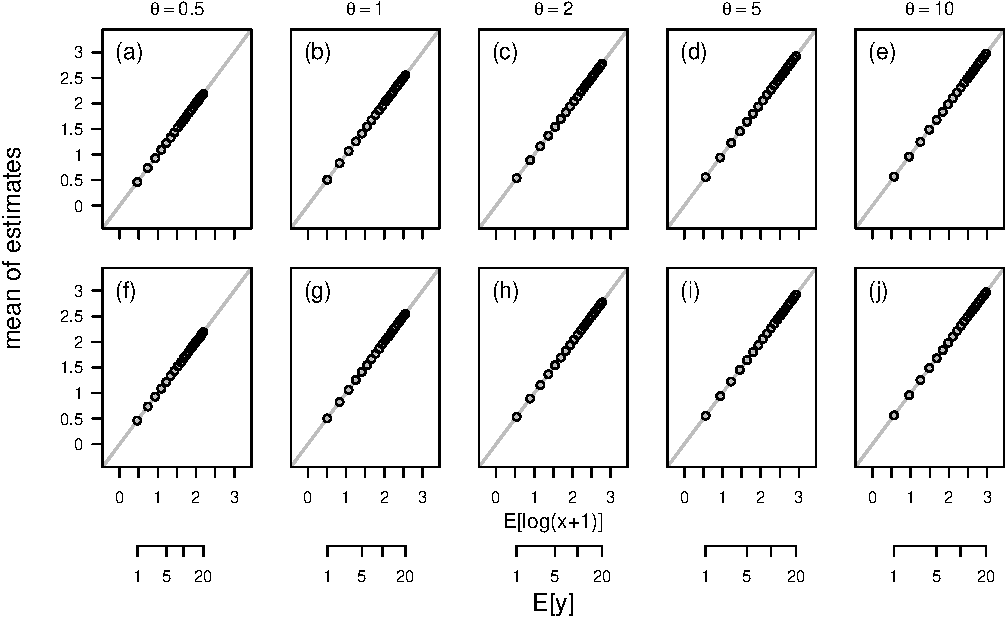
\includegraphics{revisiting_count_data_advice_files/figure-latex/biasLogPlusOne-1} 

}

\caption{Bias in estimation of the mean of negative binomial variables, transformed according to $log(y+1)$.  True simulated mean values are plotted on the x-axis, and the means of simulation results are plotted on the y-axis.  As such, points falling on the one-to-one line (grey) indicate simulation scenarios in which the analysis of $log(y+1)$ transformed data is unbiased at recovering the mean on the $log(y+1)$ scale. Plots a-e (top row) are generated from simulations where a single model estimates means of groups with true values from 1 to 20, with a common dispersion parameter or residual variance. Plots f-j (bottom row) are generated from simulations where a separate model estimates the mean and disperson parameter or residual variance for each group with a different true (simulated) mean value.}\label{fig:biasLogPlusOne}
\end{figure}

\begin{figure}[h]

{\centering 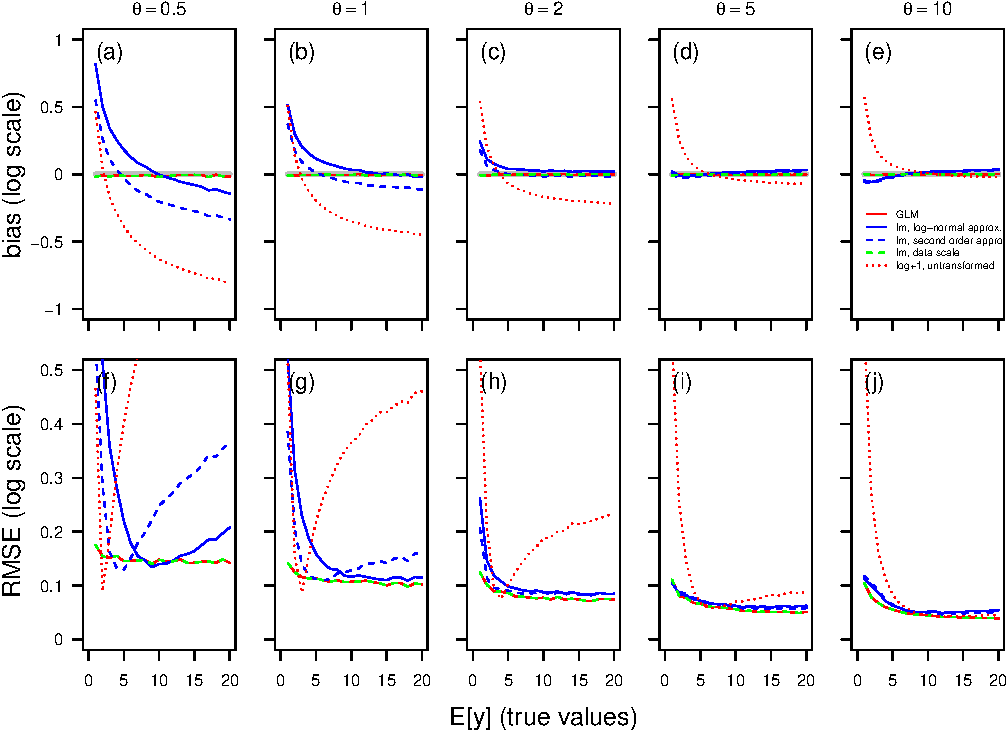
\includegraphics{revisiting_count_data_advice_files/figure-latex/biasAndRmseFigureLog-1} 

}

\caption{Bias (a-e) and overall accuracy (f-j) of inferences of the logarithm of the mean of a count variable.  Data ($n=100$) for a count variable $x$ were simulated from a negative binomial distribution with mean $E[y]$ and size parameter $\theta$.  Expressions for the two transformations of the analysis of $log(y+1)$ data are given in equations 7 and 9 of table 1. 10000 replicate simulations of each simulation were conducted and estimators of $log(E[y])$ were constructed from a suite of GLM and LM analyses.}\label{fig:biasAndRmseFigureLog}
\end{figure}

\begin{figure}[h]

{\centering 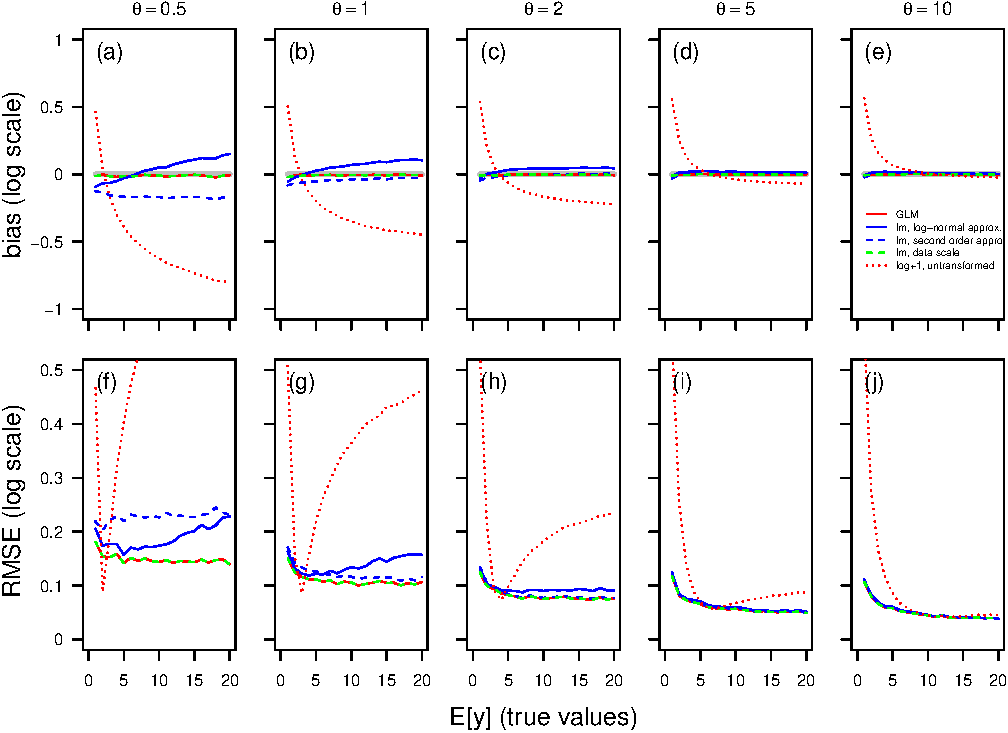
\includegraphics{revisiting_count_data_advice_files/figure-latex/biasAndRmseFigureLogSeparateModels-1} 

}

\caption{Bias (a-e) and overall accuracy (f-j) of inferences of the logarithm of the mean of a count variable.  Simulations are as for figure 2, except that each simulation involves fitting separate models for each level of the predictor variable.  Data ($n=100$) for a count variable $x$ were simulated from a negative binomial distribution with mean $E[y]$ and size parameter $\theta$.  Expressions for the two transformations of the analysis of $log(y+1)$ data are given in equations 7 and 9 of table 1.  10000 replicate simulations of each simulation were conducted and estimators of $log(E[y])$ were constructed from a suite of GLM and LM analyses.}\label{fig:biasAndRmseFigureLogSeparateModels}
\end{figure}

\clearpage
\setcounter{figure}{0} \setcounter{equation}{0} \makeatletter 
\renewcommand{\thefigure}{S.\@arabic\c@figure}
\renewcommand{\theequation}{S.\@arabic\c@equation} \makeatother

\subsection{Supplemental material}\label{supplemental-material}

\subsubsection{The negative binomial distribution:
disambiguation}\label{the-negative-binomial-distribution-disambiguation}

We used a parameterisation of the negative binomial distribution that is
common in ecology. The distribution is parameterised according to its
mean \(\mu\), and a dispersion parameter \(\theta\). The dispersion
parameter in this formulation may also be referred to as the ``size''
parameter. Given \(\mu\) (\(\mu>0\)) and \(\theta\) (\(\theta>0\)), the
probability mass function at count \(y\) is \[
p(y)=\frac{\Gamma(\theta+y)}{\Gamma(\theta)y!}\left(\frac{\theta}{\mu+\theta}\right)^\theta\left(1-\frac{\theta}{\mu+\theta}\right)^y.
\] Visualisations of the negative binomial probability distribution
functions for the ranges of \(\mu\) and \(\theta\) used in simulations
for this study are depicted in figure S.1.

Parameterised via \(\mu\) and \(\theta\), the variance of the negative
binomial distribution is \[
\sigma^2 = \mu+\frac{\mu^2}{\theta}.
\] The negative binomial converges on a Poisson distribution (such that
\(\sigma^2 = \mu\)) for large values of \(\theta\).

\subsubsection{\texorpdfstring{Derivations of estimators of \(E[y]\) and
\(log(E[y])\) in table
\ref{EstimatorsTable}}{Derivations of estimators of E{[}y{]} and log(E{[}y{]}) in table }}\label{derivations-of-estimators-of-ey-and-logey-in-table}

If the analyst is willing to assume that residuals of \(log(y+1)\)
transformed data in a linear model analysis are normally distributed,
then an estimator of the mean on the count data scale can be constructed
using the expression for the mean of a log-normal distribution. If
\(b=e^a\) and \(a\) is normally distributed according to
\(a \sim N(\mu,\sigma^2)\) (i.e., if the mean and variance of \(a\) are
\(\mu\) and \(\sigma^2\)), then the mean of \(b\) is given by \[
E[b]=e^{\mu+\frac{\sigma^2}{2}}.
\] Equation \ref{EylogLMLN} in table \ref{EstimatorsTable} uses this
relation, as well as accounting for the \(+1\) component of the
\(log(y+1)\) transformation, in order to generate an estimator of
\(E[y]\).

If it is not deemed reasonable to assume that residuals of \(log(y+1)\)
transformed data in a linear model analysis are normally distributed,
then an estimator of \(E[y]\) may be constructed as a second-order
approximation. If \(b=f(a)\), where \(f()\) is an arbitrary function,
then the mean of \(b\) may be approximated if the mean and variance of
\(a\) (which we shall again denote as \(\mu\) and \(\sigma^2\)) are
known, according to \[
E[b] \approx f(\mu) + \frac{1}{2} f^{\prime\prime}(\mu)\sigma^2,
\] where \(f^{\prime\prime}(x)\) represents the second derivative of the
function \(f()\), evaluated at \(x\). To apply the approximation, take
\(f(x)=e^x-1\) such that \(f^{\prime\prime}(x)=e^x\), applied to the
parameters estimated by model \ref{logLMmodel}, the approximation is \[
\widehat{E[y]}=e^{\alpha_{logLM}}-1+\frac{1}{2}e^{\alpha_{logLM}}\sigma^2_{logLM},
\] from which equation \ref{EylogLMTa} in table \ref{EstimatorsTable} is
obtained by algebraic simplification.

\subsubsection{Alternative scales for plotting bias and
RMSE}\label{alternative-scales-for-plotting-bias-and-rmse}

The first two supplemental figures give for absolute bias and RMSE. This
gives results in units of mean counts, rather than the log of mean
counts, as in figures 2 and 3. For simulation results where separate
means are estimated with single dispersion parameters or residual
variances across all means, absolute scale results are given in figure
S.2. Figure S.3 gives absolute scale results when separate means and
residual variances or dispersion parameters are estimated for each value
of the true mean. Figures S.4 and S.5 give the results as in figures 2
and 3, and S.2 and S.3, respectively, but on a relative scale. Relative
scale bias and RMSE is calculated by dividing the absolute bias and RMSE
(i.e., in units of counts, as plotted in figures S.2 and S.3), by the
true values of \(E[y]\).

\subsubsection{Bias and RMSE in simulations with smaller sample
size}\label{bias-and-rmse-in-simulations-with-smaller-sample-size}

Figures S.6 and S.7 give results from simulations for bias and RMSE with
sample sizes of \(n = 20\). For models simultaneously estimating means
for 20 groups, with a common residual variance or overdispersion
parameter, \(n = 20\) for each group.

\subsubsection{\texorpdfstring{Estimation variances of estimators of
\(E[y]\) and
\(log(E[y])\)}{Estimation variances of estimators of E{[}y{]} and log(E{[}y{]})}}\label{estimation-variances-of-estimators-of-ey-and-logey}

It may be useful to give expressions for estimation variances and
standard errors, at least insofar as they can be provided by standard
means. Here, we give expressions for estimation variances. Standard
errors are the square roots of these estimation variances. Then, in the
subsequent subsection, we give results demonstrating the performance of
these estimators for reflecting the true standard deviations of the
estimation variances of the estimators of \(\widehat{E[y]}\) and
\(\widehat{log(E[y])}\).

The negative binomial GLM analysis specified by equation \ref{NBmodel}
directly estimates \(log(E[y])\), and so also provides a sampling
variance via a standard error, which may be squared if desired. A
sampling variance for the estimator of \(E[y]\) using the negative
binomial GLM (eq. \ref{NBmodel}) can be constructed from the variance of
a log-normal distribution, assuming that the estimation errors of
\(\alpha_{NB}\) are approximately normally distributed. The variance of
a log-normal distribution, with parameters defined as above, is given by
\(VAR[b]=(e^\mu-1)e^{2\mu+\sigma^2}\). So, the estimation variance of an
estimate of \(E[y]\) (as estimated in eq. \ref{EyNB} in table
\ref{EstimatorsTable}) is

\begin{equation}\label{SE_EyLMNB}
VAR[\widehat{E[y]}=(e^\alpha_{NB}-1)e^{2\alpha_{NB}+VAR[\alpha_{NB}]},
\end{equation}

where \(VAR[\alpha_{NB}]\) is the estimation variance of the estimate of
\(VAR[\alpha_{NB}]\) (i.e., its standard error, squared) obtained from
the negative binomial model in equation \ref{NBmodel}.

Estimates of \(E[y]\) and \(log(E[y])\) derived from linear model-based
analysis of \(log(y+1)\) transformed data depend both on the estimate of
the mean of the \(log(y+1)\) (given by \(\alpha_{logLM}\)) and also on
the residual variance of the \(log(y+1)\) data (\(\sigma^2_{logLM}\)).
Linear model-based analysis generally yields estimation variances of
fixed parameters such as \(\alpha_{logLM}\), but not of residual
variances, i.e., of \(\sigma^2_{logLM}\). We can therefore construct
expressions for the sampling variances of \(E[y]\) and \(log(E[y])\), at
least so far estimation variance arises from imprecision in the
inference of \(\alpha_{logLM}\). The following expressions all rely on
first-order approximations for the sampling variance of a transformation
of an estimate \(\hat{b} = f(\hat{a})\), which take the general form

\begin{equation}\label{deltaMethod}
VAR[b] \approx (f^\prime(\hat{a}))^2 VAR[a],
\end{equation}

where \(VAR[b]\) is the estimation variance in some derived parameter,
\(\hat{a}\) is the estimated value of \(a\) that has some associated
estimation variance \(VAR[a]\).

Each of equations \ref{EylogLMLN} to \ref{logEylogLMTa} in table
\ref{EstimatorsTable} represents a transformation of \(\alpha_{logLM}\)
(i.e., an estimate of the mean of the \(log(y+1)\) transformed data)
into an estimate of \(E[y]\) or \(log(E[y])\). Sampling variances for
the two estimates of \(E[y]\), based on the mean of a log-normal
distribution (eq. \ref{EylogLMLN}), or using the second-order
approximation (eq. \ref{EylogLMTa}), are given, respectively, by

\begin{equation}\label{SE_EylogLMLN}
VAR[\widehat{E[y]}] = e^{2\alpha_{logLM}+\sigma^2_{logLM}}VAR[\alpha_{logLM}],~,
\end{equation}

and

\begin{equation}\label{SE_EylogLMTa}
VAR[\widehat{E[y]}] =  e^{2\alpha_{logLM}}\left(1+\frac{\sigma^2_{logLM}}{2}\right)^2VAR[\alpha_{logLM}]. ~.
\end{equation}

Sampling variances for the two estimates of \(log(E[y])\), based on the
mean of a log-normal distribution (eq. \ref{logEylogLMLN}), or using the
second-order approximation (eq. \ref{logEylogLMTa}), are given,
respectively, by

\begin{equation}\label{SE_logEylogLMLN}
VAR[\widehat{log(E[y])}]_1 =\left(\frac{e^{\alpha_{logLM}+\frac{\sigma^2_{logLM}}{2}}}{e^{\alpha_{logLM}+\frac{\sigma^2_{logLM}}{2}}-1}\right)^2VAR[\alpha_{logLM}] ~,
\end{equation}

and

\begin{equation}\label{SE_logEylogLMTa}
VAR[\widehat{log(E[y])}]_2 =  \left(\frac{e^{\alpha_{logLM}}(\sigma^2_{logLM}+2)}{e^{\alpha_{logLM}}(\sigma^2_{logLM}+2)-2}\right)^2VAR[\alpha_{logLM}]   ~.
\end{equation}

Finally, the linear model analysis of the untransformed count data
directly estimates \(E[y]\), and also directly provides a estimation
variance on the scale of the count data. A corresponding estimator of
the log of the mean may be obtained by logging this estimate. The
corresponding estimate of the estimation variance of this estimator of
the logged mean, by first order approximation, is

\begin{equation} \label{SE_logEylogLMNT}
VAR[\widehat{log(E[y])}] = \frac{1}{\alpha_{LM}^2}VAR[\alpha_{LM}]. 
\end{equation}

\subsubsection{Performance of approximations for standard errors from
OLS analyses of count
data}\label{performance-of-approximations-for-standard-errors-from-ols-analyses-of-count-data}

Standard errors of back-transformed inferences from linear model
analysis of \(log(y+1)\) transformed data performed well, closely
reflecting empirical standard deviations of estimates, in absolute terms
(i.e., in units of counts; figure S.8). In relative terms (figure S.9),
standard errors closely reflected empirical standard deviations of
estimates, providing that the data were not very highly over-dispersed
and the mean was not very low. These results are generally promising for
the back-transformations and their standard errors, as serious failures
only happen under extreme overdispersions and ranges of true means and
variances.

The linear model-based estimates from analysis of un-transformed data
behaved very differently for estimating \(log(E[y])\), depending on
whether the means of the 20 groups were estimated simultaneously or
separately (figures S.8 and S.9). The standard error depends on the
residual standard deviation of the fitted model, and this quantity will
be overestimated for small means (that have small variances), and
underestimated for large means (which have larger variances). The main
consequence of this is that standard errors perform very poorly,
especially for relatively low variance, when groups with very different
variances are analysed simultaneously. It is of note that the
simulations estimating the 20 group means simultaneously include an very
large range of variances of the count variable. The most extreme set of
variances in a single analysis (when \(\theta = 0.5\)) ranges from a
variance of 3 (when the mean is 1) to a variance of 820 (when the mean
is 20). When all means are estimated separately (i.e., for panels f-j in
figures S.8 and S.9), standard errors perform very well, essentially
equivalently to standard errors from the glm analysis.

\clearpage

\begin{figure}
\centering
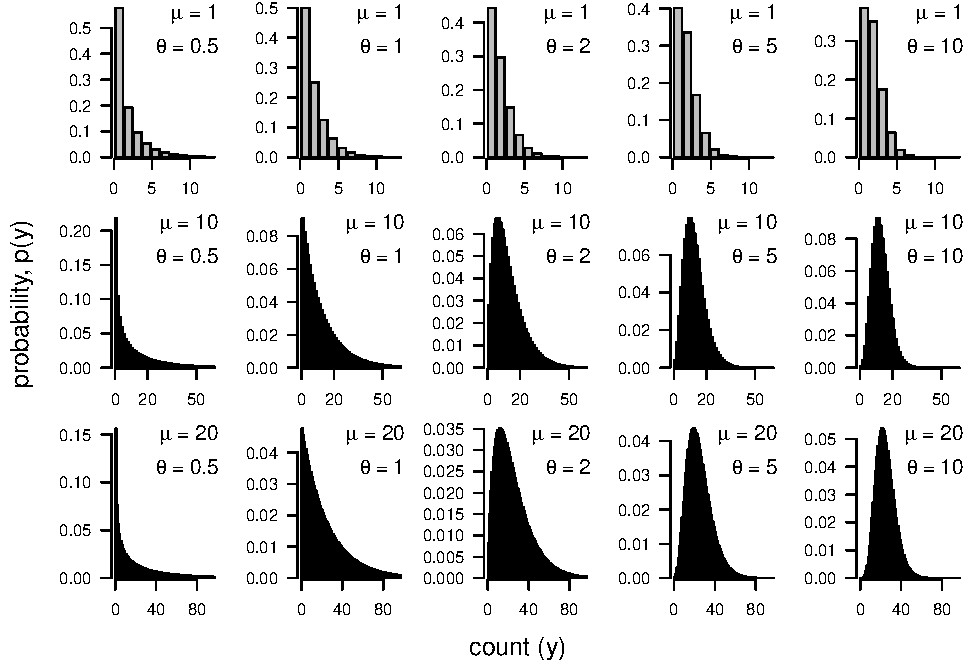
\includegraphics{revisiting_count_data_advice_files/figure-latex/negativeBinomialExamples-1.pdf}
\caption{Ranges of negative binomial distributions investigated in the
present study.}
\end{figure}

\begin{figure}[h]

{\centering 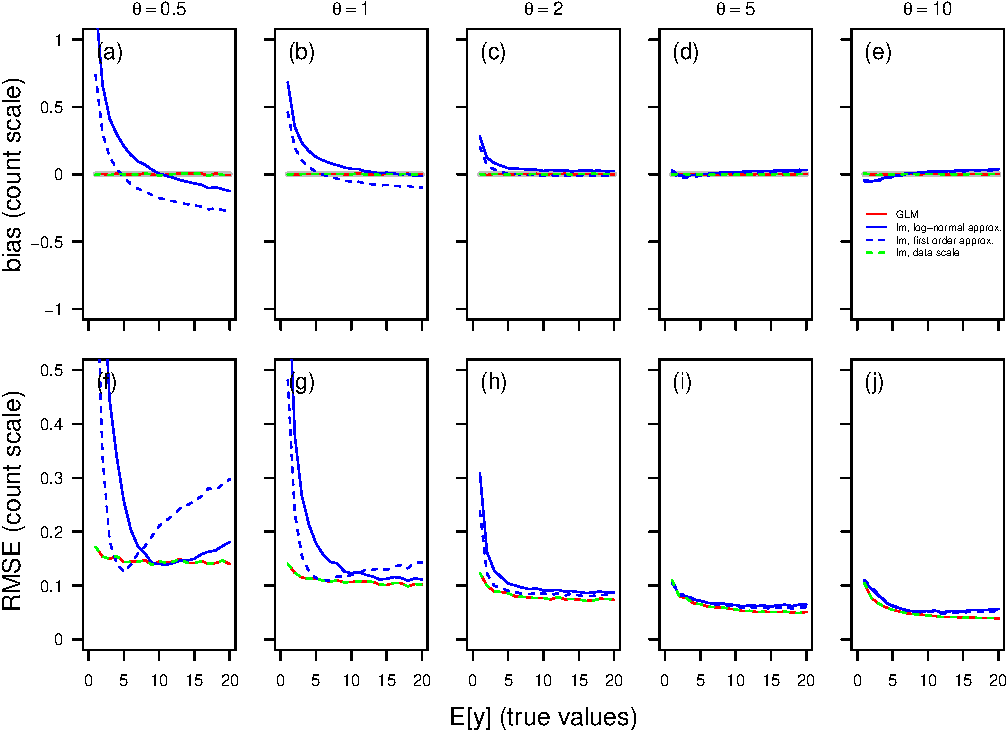
\includegraphics{revisiting_count_data_advice_files/figure-latex/SupplementAbsoluteScale-1} 

}

\caption{Bias (a-e) and overall accuracy (f-j) of inferences of the mean of a count variable.  Data ($n=100$) for a count variable $x$ were simulated from a negative binomial distribution with mean $E[y]$ and size parameter $\theta$.  Each replicate simulation yielded estimates of means for 20 groups, with true mean values of 1 to 20, and a single estimate of the dispersion parameter relevant to each model.  Expressions for the two transformations of the analysis of $log(y+1)$ data are given in equations 6 and 8 of table 1. 10000 replicate simulations of each simulation were conducted and estimators of $log(E[y])$ were constructed from a suite of GLM and LM analyses.}\label{fig:SupplementAbsoluteScale}
\end{figure}

\begin{figure}[h]

{\centering 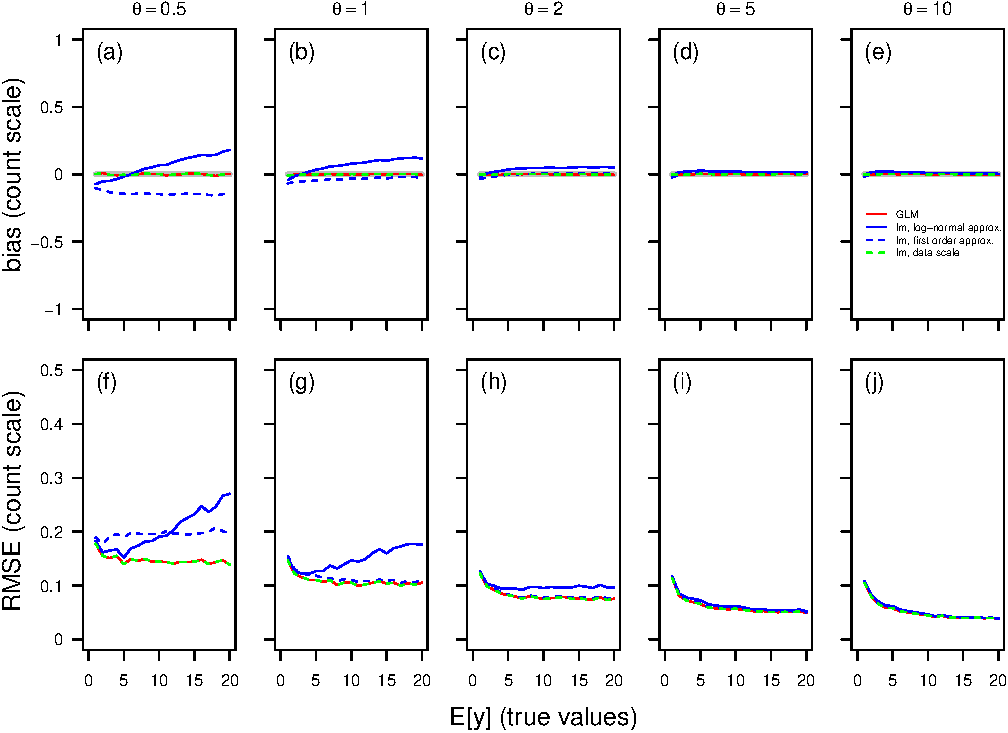
\includegraphics{revisiting_count_data_advice_files/figure-latex/SupplementAbsoluteScaleSeparateModels-1} 

}

\caption{Bias (a-e) and overall accuracy (f-j) of inferences of the logarithm of the mean of a count variable.  Data ($n=100$) for a count variable $x$ were simulated from a negative binomial distribution with mean $E[y]$ and size parameter $\theta$.   Each replicate simulation yielded separate estimates of means for 20 groups, with true mean values of 1 to 20; and corresponding separate estimates of the dispersion parameter relevant to each model.  Expressions for the two transformations of the analysis of $log(y+1)$ data are given in equations 6 and 8 of table 1. 10000 replicate simulations of each simulation were conducted and estimators of $log(E[y])$ were constructed from a suite of GLM and LM analyses.}\label{fig:SupplementAbsoluteScaleSeparateModels}
\end{figure}

\begin{figure}[h]

{\centering 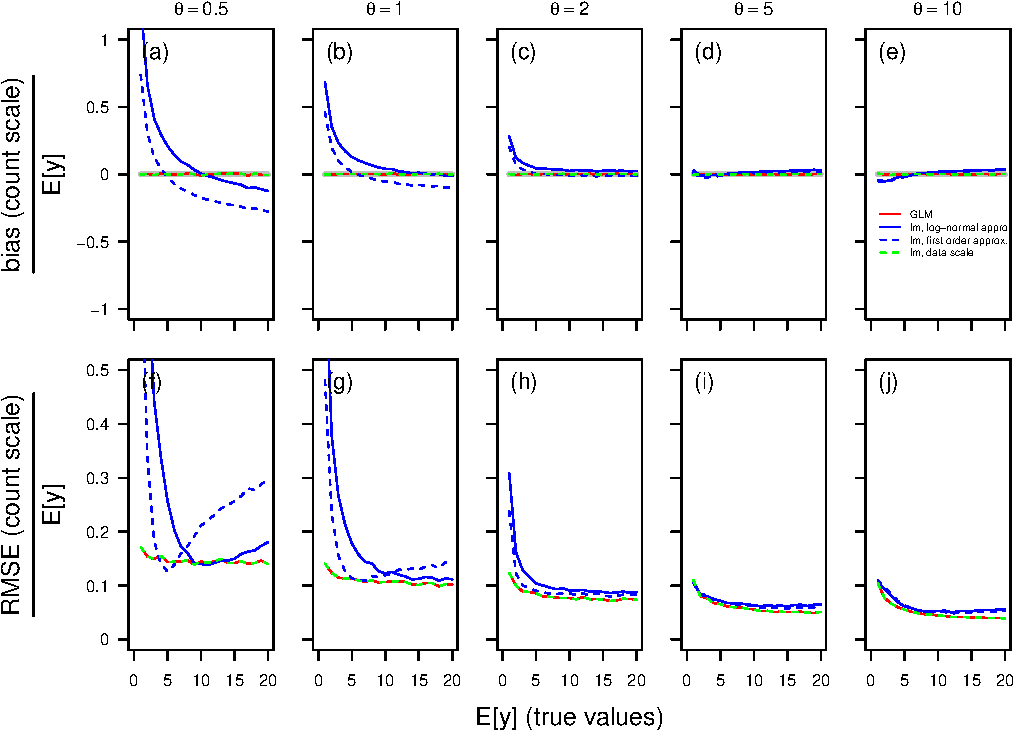
\includegraphics{revisiting_count_data_advice_files/figure-latex/SupplementRelativeScale-1} 

}

\caption{Bias (a-e) and overall accuracy (f-j) of inferences of the mean of a count variable, expressed in relation to the true mean.  Data ($n=100$) for a count variable $x$ were simulated from a negative binomial distribution with mean $E[y]$ and size parameter $\theta$.  Each replicate simulation yielded estimates of means for 20 groups, with true mean values of 1 to 20, and a single estimate of the dispersion parameter relevant to each model.  Expressions for the two transformations of the analysis of $log(y+1)$ data are given in equations 6 and 8 of table 1. 10000 replicate simulations of each simulation were conducted and estimators of $log(E[y])$ were constructed from a suite of GLM and LM analyses.}\label{fig:SupplementRelativeScale}
\end{figure}

\begin{figure}[h]

{\centering 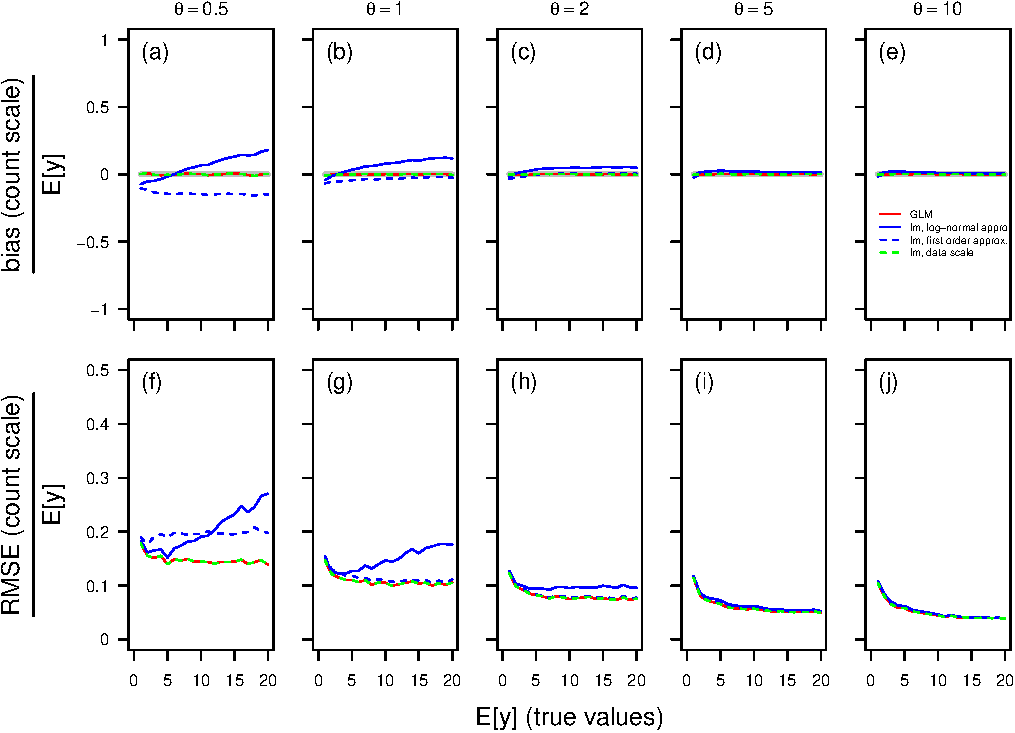
\includegraphics{revisiting_count_data_advice_files/figure-latex/SupplementRelativeScaleSeparateModels-1} 

}

\caption{Bias (a-e) and overall accuracy (f-j) of inferences of the logarithm of the mean of a count variable, expressed in relation to the tru mean.  Data ($n=100$) for a count variable $x$ were simulated from a negative binomial distribution with mean $E[y]$ and size parameter $\theta$.   Each replicate simulation yielded separate estimates of means for 20 groups, with true mean values of 1 to 20; and corresponding separate estimates of the dispersion parameter relevant to each model.  Expressions for the two transformations of the analysis of $log(y+1)$ data are given in equations 6 and 8 of table 1. 10000 replicate simulations of each simulation were conducted and estimators of $log(E[y])$ were constructed from a suite of GLM and LM analyses.}\label{fig:SupplementRelativeScaleSeparateModels}
\end{figure}

\begin{figure}[h]

{\centering 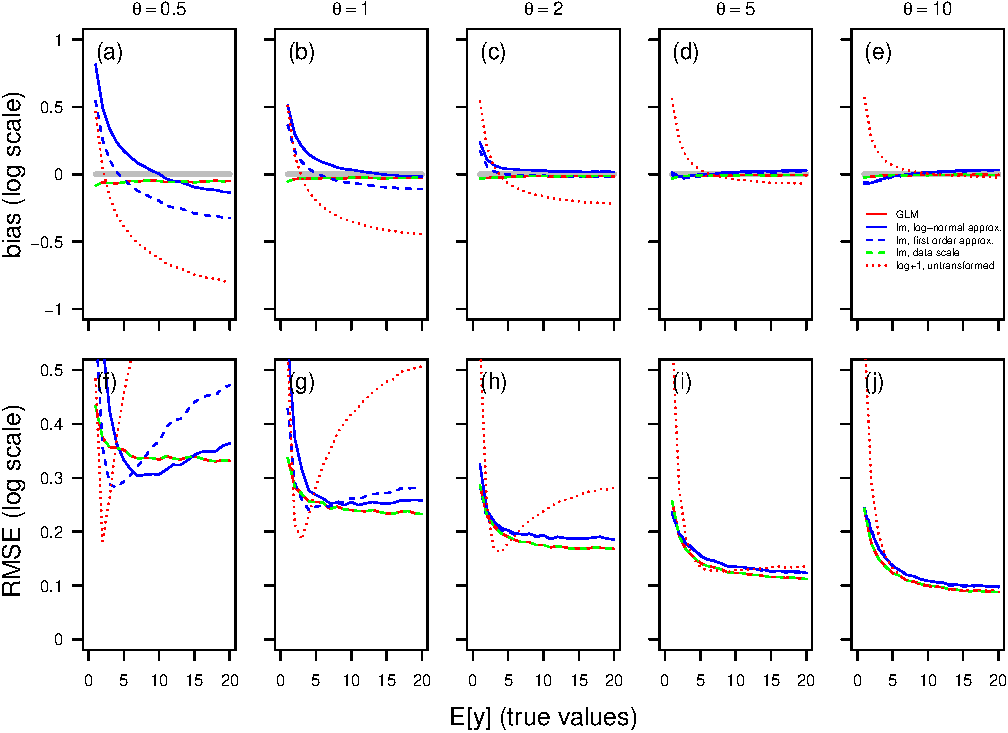
\includegraphics{revisiting_count_data_advice_files/figure-latex/biasAndRmseFigureLogSmallN-1} 

}

\caption{Bias (a-e) and overall accuracy (f-j) of inferences of the logarithm of the mean of a count variable.  Data ($n=20$, as opposed to $n=100$ as in figure 2) for a count variable $x$ were simulated from a negative binomial distribution with mean $E[y]$ and size parameter $\theta$.  Expressions for the two transformations of the analysis of $log(y+1)$ data are given in equations 7 and 9 of table 1. 10000 replicate simulations of each simulation were conducted and estimators of $log(E[y])$ were constructed from a suite of GLM and LM analyses.}\label{fig:biasAndRmseFigureLogSmallN}
\end{figure}

\begin{figure}[h]

{\centering 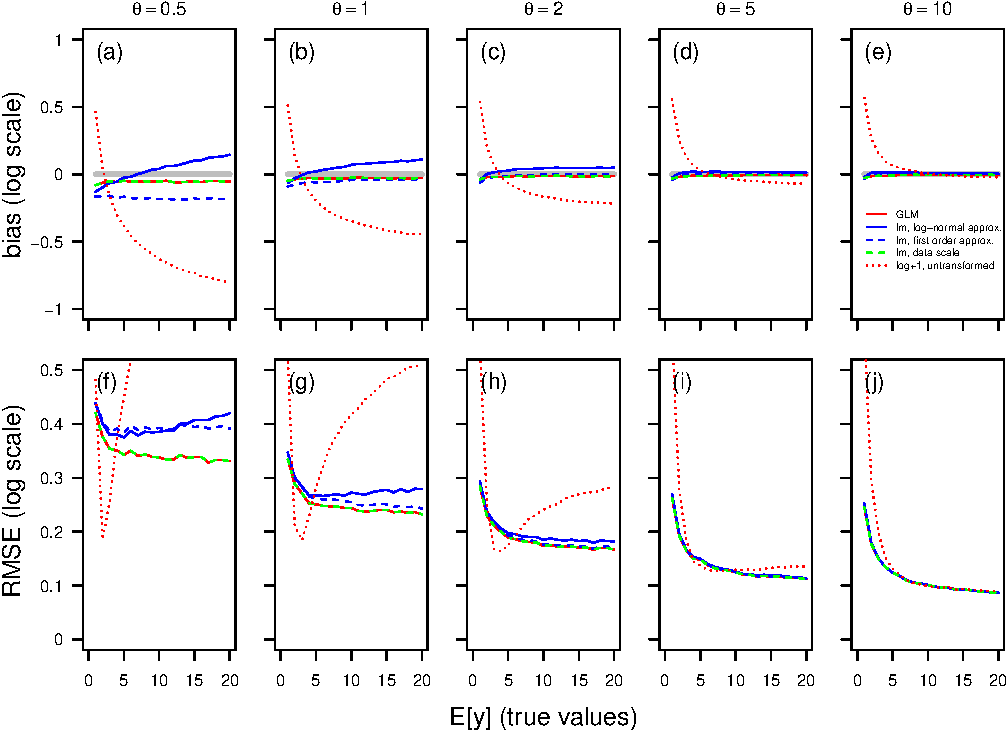
\includegraphics{revisiting_count_data_advice_files/figure-latex/biasAndRmseFigureLogSeparateModelsSmallN-1} 

}

\caption{Bias (a-e) and overall accuracy (f-j) of inferences of the logarithm of the mean of a count variable.  Separate models were fitted for each factor level (each with a differen true mean).  Data ($n=20$, as opposed to $n=100$ as in figure 3) for a count variable $x$ were simulated from a negative binomial distribution with mean $E[y]$ and size parameter $\theta$.  Expressions for the two transformations of the analysis of $log(y+1)$ data are given in equations 7 and 9 of table 1.  10000 replicate simulations of each simulation were conducted and estimators of $log(E[y])$ were constructed from a suite of GLM and LM analyses.}\label{fig:biasAndRmseFigureLogSeparateModelsSmallN}
\end{figure}

\begin{figure}[h]

{\centering 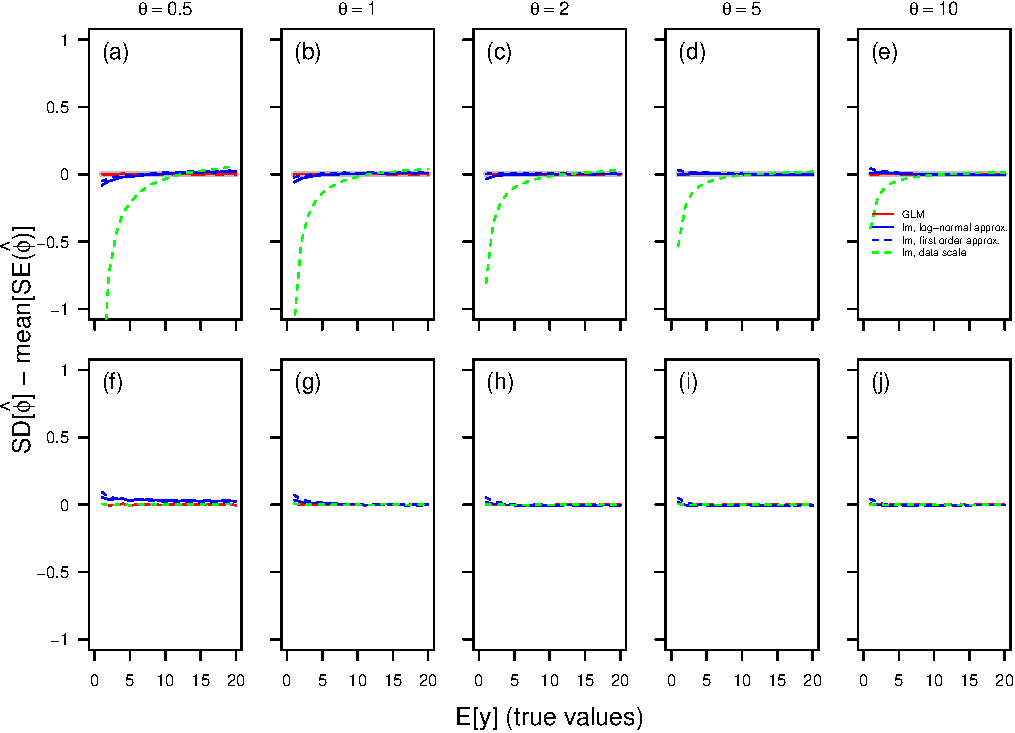
\includegraphics{revisiting_count_data_advice_files/figure-latex/SEPerformanceFigureLog-1} 

}

\caption{The validity of standard errors of estimates of the log of the mean of a count variable (i.e., $\phi=log(E[y])$), evaluated by the difference between the empirical standard deviation of estimates across simulations, and the mean standard error taken across simulations.  (a-e) show results when estimates groups with true values of $log(E[y])$ between 1 and 20 are inferred simultaneously, and (f-j) show results when $log(E[y])$ for each group is estimated separately. Data for a count variable $y$ and a predicor variable $x$ with twenty groups ($n=100$ per group) with true means from 1 to 20, were simulated from a negative binomial distribution with mean $E[y]$ and size parameter $\theta$, and analysed with models estimating twenty location parameters and a single dispersion parameter (parts a-e) or with a separate model for each level of $x$ (parts f-g. 10000 replicate simulations of each simulation were conducted and estimators of $log(E[y])$ were constructed from a suite of GLM and LM analyses.}\label{fig:SEPerformanceFigureLog}
\end{figure}

\begin{figure}[h]

{\centering 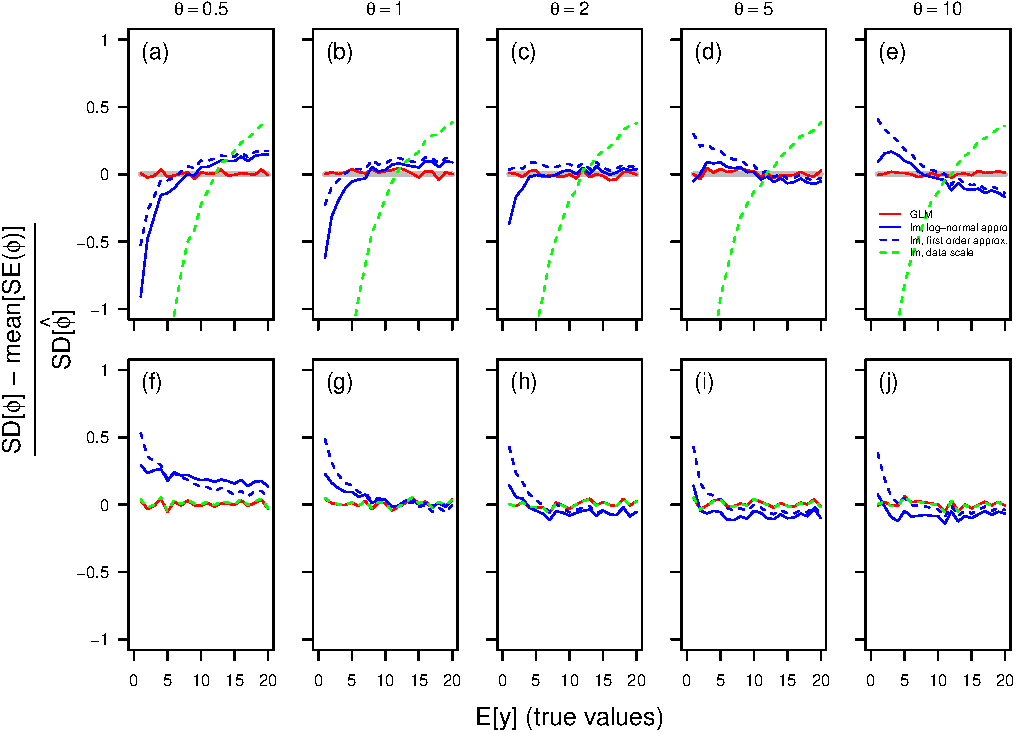
\includegraphics{revisiting_count_data_advice_files/figure-latex/SEPerformanceFigureLogRelative-1} 

}

\caption{The validity of standard errors of estimates of the log of the mean of a count variable (i.e., $\phi=log(E[y])$), evaluated by the difference between the empirical standard deviation of estimates across simulations, and the mean standard error taken across simulations, and expressed in relation to the true standard deviation.  (a-e) show results when estimates groups with true values of $log(E[y])$ between 1 and 20 are inferred simultaneously, and (f-j) show results when $log(E[y])$ for each group is estimated separately. Data for a count variable $y$ and a predicor variable $x$ with twenty groups ($n=100$ per group) with true means from 1 to 20, were simulated from a negative binomial distribution with mean $E[y]$ and size parameter $\theta$, and analysed with models estimating twenty location parameters and a single dispersion parameter (parts a-e) or with a separate model for each level of $x$ (parts f-g. 10000 replicate simulations of each simulation were conducted and estimators of $log(E[y])$ were constructed from a suite of GLM and LM analyses.}\label{fig:SEPerformanceFigureLogRelative}
\end{figure}


\end{document}
